\documentclass[12pt,a4paper,twoside]{article}
\RequirePackage[T1]{fontenc}
\RequirePackage{times}
\RequirePackage[utf8]{inputenc}
\RequirePackage[polish]{babel}

\RequirePackage{comment}

\RequirePackage{a4wide}
\RequirePackage{longtable}
\RequirePackage{multicol}
\RequirePackage{url}

\usepackage[pdftex]{graphicx}

% $Id: sad-template.tex,v 1.1.1.1 2001/10/30 17:49:15 robmar Exp $
\author{Piotr Czubak, Marcin Kanclerz, Paweł Kozłowski, Filip Mazowiecki}
\title{Software Architecture Document projektu Quall na ZPP 09/10}
\begin{document}

\maketitle

\newpage

\tableofcontents

\newpage

% Note: The following template is provided for use with the Rational
% Unified Process. Text enclosed in square brackets and displayed in blue
% italics (style=InfoBlue) is included to provide guidance to the author
% and should be deleted before publishing the document. A paragraph entered
% following this style will automatically be set to normal (style=Body
% Text).

% To customize automatic fields (which display a gray background when
% selected), select File>Properties and replace the Title, Subject and
% Company fields with the appropriate information for this document.
% After closing the dialog, automatic fields may be updated throughout the
% document by selecting Edit>Select All (or Ctrl-A) and pressing F9, or
% simply click on the field and press F9. This must be done separately
% for Headers and Footers. Alt-F9 will toggle between displaying the
% field names and the field contents. See Word help for more information
% on working with fields.] 


\section{Wprowadzenie}

% The introduction of the Software Architecture Document should provide an
% overview of the entire Software Architecture Document. It should include
% the purpose, scope, definitions, acronyms, abbreviations, references, and
% overview of the Software Architecture Document.

\subsection{Cel}

% EXAMPLE:
% This document provides a comprehensive architectural overview of the
% system, using a number of different architectural views to depict different
% aspects of the system. It is intended to capture and convey the
% significant architectural decisions which have been made on the system.

% This section defines the role or purpose of the Software Architecture
% Document, in the overall project documentation, and briefly describes the
% structure of the document. The specific audiences for the document should
% be identified, with an indication of how they are expected to use the
% document.

Ten dokument przedstawia ogólny przegląd architektury Quall, wykorzystując kilka różnych perspektyw, aby uchwycić i przekazać najistotniejsze decyzje architektoniczne. Strukturę dokumentu oparto na modelu 4 + 1:

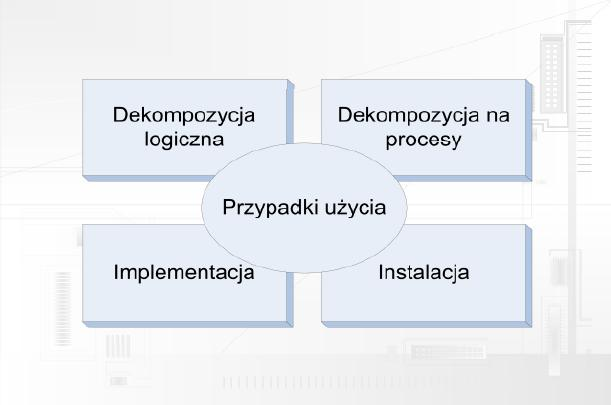
\includegraphics{pics/struktura.jpg}

Software Architecture Document jest adresowany zarówno do projektantów jak i programistów.

\subsection{Zakres}

% A brief description of what the Software Architecture Document applies
% to; what is affected or influenced by this document.

Dokument dotyczy projektu Quall - gry z gatunku Third Person Shooter.

\subsection{Definicji i skróty}

% This subsection should provide the definitions of all terms, acronyms,
% and abbreviations required to properly interpret the Software
% Architecture Document.  This information may be provided by reference to
% the project Glossary.

\begin{itemize}
\item SAD - Software Architecture Document, czyli dokument prezentujący architekturę systemu.
\item TPS - Third Person Shooter, typ gry komputerowej w której sterowaną postać obserwujemy zza jej pleców, a walka z przeciwnikiem polega na próbie zabicia go strzelając do niego z różnego rodzaju broni.
\end{itemize}

%\subsection{Załączniki}

% This subsection should provide a complete list of all documents
% referenced elsewhere in the Software Architecture Document. Each
% document should be identified by title, report number (if applicable),
% date, and publishing organization. Specify the sources from which the
% references can be obtained. This information may be provided by reference
% to an appendix or to another document.

\subsection{Omówienie reszty dokumentu}

% This subsection should describe what the rest of the Software
% Architecture Document contains and explain how the Software Architecture
% Document is organized.

Pełny obraz projektu Quall gwarantują nastepujące sekcje SADu:

% tu niech kazdy dodaje do itemiza to co sam napisal

\begin{itemize}
\item Sekcja 2 - opis prezentacji architektury systemu w poniższym dokumencie.
\item Sekcja 3 - opis założeń i zależności.
\item Sekcja 4 - opis przypadków użycia.
\item Sekcja 5 - opis warstwy logicznej projektu.
\item Sekcja 6 - opis podziału projektu na procesy oraz komunikacji między nimi.
\item Sekcja 7 - opis instalacji systemu.
\item Sekcja 8 - opis implementacji systemu.
\item Sekcja 9 - historia zmian dokumentu.
\end{itemize}

\section{Prezentacja architektury systemu}

% This section describes what software architecture is for the current
% system, and how it is represented. Of the Use-Case, Logical, Process,
% Deployment, and Implementation Views, it enumerates the views that are
% necessary, and for each view, explains what types of model elements it
% contains.

Zgodnie z modelem 4 + 1 architektura zaprezentowana jest w następujących ujęciach:

\begin{itemize}
\item Dekompozycja logiczna - omawia wymagania funkcjonalne, prezentuje model obiektowy projektu i realizację kluczowych przypadków użycia, jest zaadresowana do projektantów.
\item Dekompozycja na procesy - zaadresowana do integratorów, omawia zagadnienia związane ze współbieżnoscią w grze Quall. 
\item Implementacja - skierowana do programistów, opisuje warstwy architektury i podsystemy aplikacji, zawiera diagram warstw.
\item Instalacja - opisuje przeniesienie systemu na sprzęt komputerowy, skierowana jest do osób odpowiedzialnych za wdrożenie.
\item Przypadki użycia - prezentują funkcjonalność systemu. Są skierowane do wszystkich osób mających wpływ na wymagania oraz do użytkowników.
\end{itemize}

\section{Założenia i zależności}

% This section describes the software requirements and objectives that have
% some significant impact on the architecture, for example, safety,
% security, privacy, use of an off-the-shelf product, portability,
% distribution, and reuse. It also captures the special constraints that
% may apply: design and implementation strategy, development tools, team
% structure, schedule, legacy code, and so on.

\begin{itemize}
\item Asymetryczna architektura klient-serwer - do wymiany komunikatów między sobą klient i serwer będą miały stworzone dodatkowe wątki, co nie będzie zauważalnie spowalniało działania całej aplikacji.
\item Stabilność - serwer powinnien być w stanie obsłużyc kilkunastu graczy jednocześnie, bez konieczności częstego resetowania.
\item Wydajność - aby rozgrywka przebiegała płynnie czas oczekiwania na odpowiedź serwera nie powinnien przekraczać 150 milisekund.
\end{itemize}

Aplikacja kliencka będzie napisana w języku C++, jest pisana z myślą o platformie Windows. Do stworzenia projektu korzystamy z narzędzia Microsoft Visual Studio 2008 Professional. Serwer także zostanie napisany w C++, głównie ze względu na znaczenie wydajności i możliwości obsługi wielu graczy naraz. Harmonogram prac będzie ustalany przy pomocy serwisu Assembla (www.assembla.com). Marcin Kanclerz jest kierownikiem projektu, zatem z wszelkimi wątpliwościami członkowie zespołu będą mogli zwracać się do niego.\\
\\
Wszelkie kwestie związane z grafiką i jej wyświetlaniem zostaną obsłużone przez open-source'owy silnik graficzny Ogre. Obliczanie wzajemnego położenia obiektów na planszy oraz kolizji między nimi będzie możliwe dzięki wykorzystaniu silnika fizycznego Bullet. Zdarzenia związane z obsługą wejścia (klawiatura i mysz) będą obsługiwane przez system OIS, a związane z obsługą dźwięku przez OpenAL.

\section{Przegląd przypadków użycia i ich realizacja}

% This section lists use cases or scenarios from the use-case model if they
% represent some significant, central functionality of the final system, or
% if they have a large architectural coverage - they exercise many
% architectural elements, or if they stress or illustrate a specific,
% delicate point of the architecture.
% This section illustrates how the software actually works by giving a few
% selected use-case (or scenario) realizations, and explains how the
% various design model elements contribute to their functionality.

\subsection{Uruchomienie gry}
Początkowa faza każdego gracza. Gracz uruchamia sobie aplikację kliencką i zostanie mu wyświetlone odpowiednie menu, w którym będzie mógł wybrać: Gra w trybie CTF, zmiana ustawień, wyjście. Każdy z tych przypadkow zostanie opisany poniżej.
\\
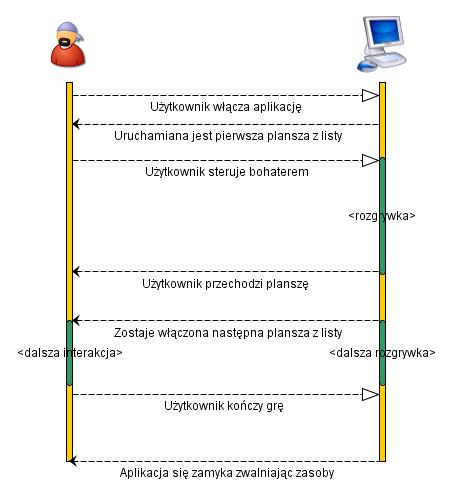
\includegraphics{pics/WejscieDoGry.jpg}

\subsection{Zmiana ustawień}
Każdemu graczowi po wybraniu zmiany ustawień wyświetli się odpowiednie podmenu. Gracz będzie miał możliwość modyfikowania parametrów dotyczących grafiki, dźwięku lub sterowania. Przy grafice i dźwięku będzie odpowiednik pasek na którym gracz będzie mógł wybrać rozdzielczość i głośność w grze. Po kliknieciu w sterowanie graczowi wyświetli się kolejne podmenu, w którym będzie mógł zdefiniować jakimi przyciskami chce sterować w trakcie gry. Domyślnie będą to: przyciski W, S, A, D do poruszania się,lewy przycisk myszki do wykonania akcji, spacja do skakania i liczby 1-4 do zmiany broni. Będą odpowiednie przyciski OK i anuluj żeby gracz mógł w każdej chwili zapisać zmiany w ustawieniach albo powrócić bez zmian do poprzedniego menu.

\subsection{Wyjście}
Po wybraniu tego gracz zamknie aplikację.

\subsection{Gra w trybie CTF}
Po wybraniu tego graczowi zostanie wyswietlone miejsce na wpisanie IP serwera, z którym chce się połączyć. Jeśli IP serwera zostało wprowadzone poprawnie i serwer prawidłowo przydzielił graczowi plansze wyświetli się tryb rozgrywki opisany poniżej. W przeciwnym wypadku gracz powróci do poprzedniego menu.

\subsection{Tryb rozgrywki}
Gracz dostanie własną postać - kulkę, którą będzie sie poruszał po planszy. Zostanie przydzielony do jednej z drużyn zgodnie z trybem rozgrywki CTF. W trakcie gry gracz będzie mógł wyjśc do menu rozgrywki przez wciśnięcie Esc, gdzie będą cztery dla niego cztery możliwości do wyboru: Powrót do gry, Zmiana ustawień, Wyjście do Menu głównego, Wyjście z gry. Każda z tych możliwości jesli zostanie wybrana przekieruje gracza w odpowiednie miejsce - tzn Powrót do gry - wróci do trybu rozgrywki, Wyjście do Menu głównego spowoduje, że gracz wyjdzie z tej rozgrywki i wróci do menu głównego gry, Wyjście z gry zamknie całą aplikację kliencką, a Zmiana ustawień spowoduje wejście do menu zmiany ustawień. Jeśli administrator przerwie grę, gracz zostanie wyrzucony do głównego menu i zostanie o tym poinformowany odpowiednim komunikatem.

W trybe rozgrywki gracz będzie miał w lewym górnym rogu wyświetlone statystyki dotyczące punktów za zdobycie flag oraz liczniki fragów dla poszczególnych drużyn i graczy. W lewym dolnym rogu jest wyświetlane ile graczowi zostało życia (0-100) oraz jakiej wielkości jest kulka. Rozmiary kulki zależa od tego ile zostało życia graczowi. Poza tym gracz będzie mógł poruszać się po planszy. Jest to podzielone na akcje: Ruch, Obrót, Strzał, Kolizja które zostaną opisane w rozdziałach poniżej.

\subsection{Ruch}
Ruch będzie się odbywał domyślnie za pomocą WSADa na klawiaturze i klawiszem do skakania np spacją. Ruch będzie polegał na tym że kulka będzie się toczyła w wybranym kierunku i ewentualnie skakała. W zależności od wielkości kulki gracz będzie miał dostęp do niektórych dziur w planszy, które na przykład będą jakąś drogą na skróty. Obrót w jakim gracz się znajduje definiuje kierunek na płaszczyźnie, w którym będzie się poruszał. W trakcie ruchu może dojść do zderzenia ze ścianą, innym graczem lub flagą - zostanie to opisane w rozdziale Kolizja.

\subsection{Obrót}
Gracz w trakcie gry będzie mógł też sie obracać. Do tego będzie służyła myszka i w ten sposób gracz może wyznaczyć stronę w którą będzie sie ruszał. Na środku widoku będzie celownik, który będzie pokazywał w którą stronę gracz sie bedzie ruszał oraz, w którą będzie strzelał.

\subsection{Strzał}
Za pomocą wciśnięcia specjalnego przycisku (domyślnie lewy przycsik myszki) gracz będzie mógl wykonać strzał. Jeśli przytrzyma ten przycisk to w odpowiednich odstępach dla danej broni będą robiły się kolejne strzały. Do tego gracz potrzebuje mieć broń z amunicją, wtedy po kliknięciu zostanie wystrzelony pocisk w kierunku w jakim gracz jest obrócony. Odpowiednimi przyciskami (domyślnie 1-4) gracz może wybierać sobie bronie, które do tej pory zebrał. W prawym dolnym rogu będzie wyświetlone ile jest amunicji dla danej broni, po każdym strzale zostanie zmniejszona o 1. Po strzale może dojść do kolizji między wystrzelonym pociskiem a ścianą lub innym graczem. Jest to opisane w rozdziałach niżej. Jeśli w wyniku strzału zabije innego gracza zostaną zaktualizowane statystyki wyświetlane w lewym górnym rogu.

\subsection{Kolizja}
Zderzenie ze sobą dwóch elementów będzie nazywane kolizją. Może do niej dojść na różne sposoby i między różnymi obiektami. Dokładny opis poszczególnych przypadków jest w poniższych rozdzialach:

\subsubsection{Pocisku}
Ta kolizja występuje jesli jeden z graczy trafił drugiego strzałem z broni. Wtedy w wyniku tej kolizji pocisk znika (ew. emituje jakąś imitacje wybuchu), a trafionemu graczowi zostanie odjęta odpowiednia ilośc życia. Jeśli gracz przekroczy pewien próg życia zostanie też jego kulka zmniejszona do odpowiedniego rozmiaru. Za każdym razem jak gracz zostanie postrzelony będzie efekt graficzny - ekran w pewnym miejscu stanie się bardziej czerwony żeby gracz się zorientował że jest trafiany. Jesli gracz straci całe życie i zostanie mu 0, to nie będzie mógł nic robić przez pewien czas, a potem jesgo postać zostanie przywrócona w pewnym miejscu na planszy z pełnym życiem i bez broni.

\subsubsection{Dwóch graczy}
Ta kolizja występuje jeśli kulki dwóch graczy zderzą się ze sobą. Wtedy kulki odbiją się od siebie i odlecą w odpowiednich kierunkach.

\subsubsection{Gracza z elementem świata}
Ta kolizja występuje kiedy gracz wpadnie na jakiś stały element planszy - np plansze. Wtedy kulka gracza sama się obije w odpowiednim kierunku pozostawiając nienaruszoną część świata.

\subsubsection{Gracza z flagą}
Na planszy sa dwie flagi. Z punktu widzenia gracza jedna należy do jego drużyny, a druga do przeciwnej. Domyślnie znajdują się one w specjalnym miejscy dla każdej z nich co będzie się nazywać bazą drużyny. Jeśli gracz wejdzie we flage przeciwnika, która znajduje się w jego bazie lub porzucona gdzie indziej na planszy to będzie ją miał na sobie. Wtedy jeśli uda mu się dojść do swojej bazy drużyna zdobędzie punkt. Jeśli po drodze zostanie zabity flaga wypadnie i będzie leżała w miejscu gdzie gracz został zabity. Jeśli gracz wejdzie w swoją flagę, która znajduje się gdzieś poza jego bazą to ta flaga zostanie automatycznie przywrócona na swoje domyślne miejsce. Jeśli wejdzie na nią jak ona będzie w bazie to będzie to zwykłe zachowanie jak podczas zderzenia z elementem świata.

\subsubsection{Gracza z Bonusem}
Na planszy znajdują się dwa rodzaje bonusów. Życie i broń. W wyniku kolizji gracza z życiem zostanie uzupełnione jego życie o pewną ilość przy czym tak, że nigdy nie przekroczy to 100. Zetknięcie z bronią powoduje że gracz wchodzi w posiadanie danej broni jesli jej nie miał oraz, uzupełniona zostaje jego amunicja o pewną ilość naboji. Po takiej kolizji z graczem dany bonus znika z planszy. Bonusy są rozmieszczane co jakiś czas w losowych miejscach na planszy. 

\subsection{Wejście dla administratora}
Oddzielne wejście do gry będzie miał administrator. Po uruchomienu aplikacji administratora zostanie my wyświetlone specjalne menu, gdzie będzie miał możliwe opcje: załaduje plansze, wyjście. Wyjście powoduje, że aplikacja administratora zostanie zamknięta. Załadowanie planszy powoduje że otwiera sie kolejne menu gdzie administrator może załadować jakąś plansze ze swojego dysku. Jeśli plansza nie załaduje się pomyślnie to administrator zostanie w tym samym menu tylko wyświetli się odpowiedni komunikat o błędzie. Jeśli ładowanie przejdzie pomyślnie to serwer pozostanie w oczekiwaniu na zgłaszających się graczy do gry żeby ich dodać. Administrator będzie mógł przerwać działanie co spowoduje że wszyscy zalogowani klienci zostaną wyrzuceni z niej, a administrator wejdzie do poprzedniego menu.

\section{Dekompozycja logiczna systemu}

% This section describes the architecturally significant parts of the
% design model, such as its decomposition into subsystems and packages.
% And for each significant package, its decomposition into classes and
% class utilities. You should introduce architecturally significant classes
% and describe their responsibilities, as well as a few very important
% relationships, operations, and attributes.

Quall jest grą sieciową opartą o architekturę klient-serwer. W aplikacji klienckiej wyróżnić można cztery warstwy logiczne. Serwer z racji dość prostej budowy posiada tylko dwie warstwy.

\subsection{Omówienie}

% This subsection describes the overall decomposition of the design model
% in terms of its package hierarchy and layers.

\subsubsection{Aplikacja kliencka}
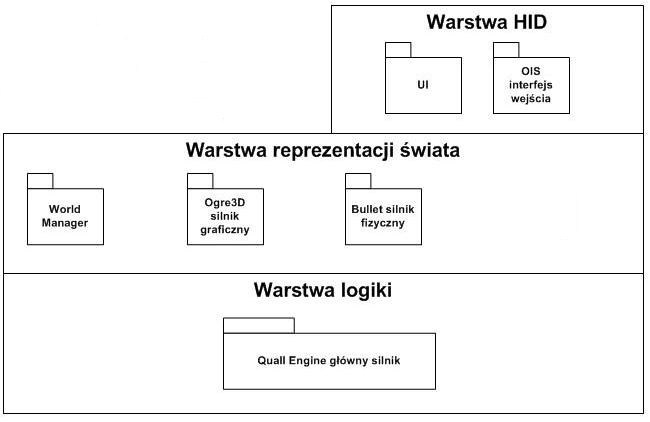
\includegraphics{pics/LogicalViewClient.jpg}
\begin{itemize}
\item Warstwa HID - warstwa odpowiedzialna za zbieranie danych z urządzeń wejścia oraz propagowanie ich do warstwy logiki bądź reprezentacji świata w odpowiedniej postaci.
\item Warstwa logiki - warstwa inicjująca całą aplikację i rozdzielająca pracę pomiędzy pozostałe warstwy, opisująca logikę samej gry, informująca warstwę sieci o aktualnym stanie gry.
\item Warstwa reprezentacji świata - warstwa przekładająca stan gry na reprezentację świata poprzez realizację fizyki obiektów, udźwiękowienie oraz wizualizację, bezpośredni dostęp do niej mają warstwy sieci oraz HID, co pozwala im bezpośrednio zmieniać aktualny świat.
\item Warstwa sieci - warstwa odpowiedzialna za połączenie z serwerem oraz przesyłanie danych dotyczących stanu gry do serwera i odbieranie z serwera wszelkich informacji o pozostałych graczach oraz propagowanie ich do warswy logiki bądź reprezentacji świata w odpowiedniej postaci.
\end{itemize}

\subsubsection{Serwer dedykowany}
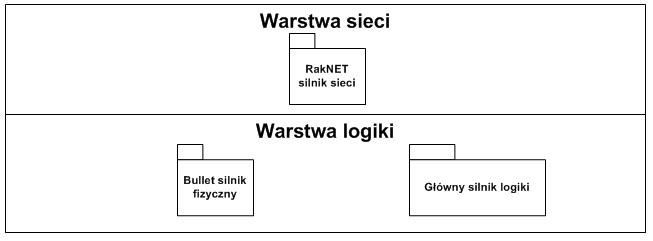
\includegraphics{pics/LogicalViewServer.jpg}
Serwer stanowi dwumodułową aplikację, gdzie jeden moduł jest odpowiedzialny za utrzymywanie wielowątkowej komunikacji z klientami, zaś drugi odpowiedzialny jest za przeliczanie fizyki gry. Wynik obliczeń rozsyłany jest do wszystkich klientów.

\subsection{Najważniejsze komponenty}

% For each significant package, include a subsection with its name, its
% brief description, and a diagram with all significant classes and
% packages contained within the package. 

% For each significant class in the package, include its name, brief
% description, and, optionally a description of some of its major
% responsibilities, operations and attributes.

\subsubsection{OIS (interfejs wejścia)}
Komponent w sposób bezpośredni przekłada zdarzenia pochodzące z klawiatury oraz myszki na dane w postaci łatwej do przetworzenia dla dalszych modułów.
\subsubsection{Quall Engine}
Komponent zarządzający stanem gry, generowaniem odpowiednich akcji na podstawie dostarczonych danych przez warstwę sieci oraz wejścia, jak również wysokopoziomową logiką gry.
\subsubsection{World Manager}
Komponent utrzymujący synchronizację pomiędzy światem widzianym (silnik graficzny) oraz światem fizycznym (silnik fizyczny). Realizujący również niskopoziomową logikę gry (np. dźwięk) na podstawie zdarzeń generowanych przez system kolizji.
\subsubsection{Silnik sieci w aplikacji klienckiej}
Komponent odpowiedzialny za utrzymanie połączenia z serwerem oraz filtrowanie i synchronizację przesyłanych danych w obydwu kierunkach.
\subsubsection{Silnik sieci w serwerze}
Komponent odpowiedzialny za asynchroniczną, wielowątkową obsługę połączeń z klientami.
\subsubsection{Silnik serwera}
Komponent realizujący synchronizację fizyki pomiędzy klientami. Serwer będzie odbierał akcje klienta następnie wyliczał zmiany położeń poszczególnych obiektów i odsyłał wyniki do klientów.\\
\\
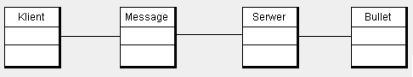
\includegraphics{pics/classdiagram.png}

\section{Dekompozycja na procesy}

% This section describes the system's decomposition into lightweight
% processes (single threads of control) and heavyweight processes
% (groupings of lightweight processes). Organize the section by groups of
% processes that communicate or interact. Describe the main modes of
% communication between processes, such as message passing, interrupts, and
% rendezvous.

Quall dzieli się na aplikację kliencką oraz serwer dedykowany.

\subsection{Aplikacja kliencka}

\begin{itemize}
\item Główny wątek gry - obsługa głównej pętli, która renderuje świat gry oraz obsługuje bezustanną jego modyfikację przez system wejścia, silnik fizyczny i warstwę sieciową.
\item Wątek obsługujący wejście - obsługa systemu wejścia, komunikacja za pomocą zdarzeń z głównym wątkiem gry.
\item Wątek warstwy sieciowej - obsługa informacji przychodzących z serwera, które opisują interakcję między poszczególnymi graczami. Komunikacja za pomocą przerwań z głównym wątkiem gry.
\end{itemize}

\subsection{Serwer dedykowany}

\begin{itemize}
\item Główny wątek serwera - obsługa zależności między poszczególnymi graczami oraz połączenie tego z obliczeniami zwróconymi przez silnik fizyczny.
\item Wątek komunikacyjny - stworzony dla każdego klienta, który podłączył się do serwera, komunikacja za pomocą zsynchronizowanych komunikatów.
\end{itemize}

\subsection{Protokół komunikacyjny}
Komunikacja pomiędzy aplikacją kliencką a serwerem dedykowanym odbywa sie za pomocą protokołu TCP ponieważ istotne jest żeby wszystkie dane docierały do swoich adresatów. Po obu stronach wymianie komunikatów obsługują oddzielne wątki, które na podstawia wymienianych informacji uaktualniają swoje silniki fizyczne i graficzne dzięki dostępowi do klasy WorldManager. \\
\newline
Klient wysyła do serwera 2 rodzaje komunikatów: o wystrzelonych pociskach i o swojej pozycji na planszy. Na każdy komunikat z informacją o pozycji serwer odpowiada wysyłając współrzędne pozostałych graczy. Ponadto serwer może poinformować klienta o zderzeniach (jakiego rodzaju zderzenia będą wykrywane po stronie serwera, a które po stronie klienta, będzie ustalone na podstawie testów). Łącznie więc istnieją 3 rodzaje komunikatów, każdy z nich jest reprezentowany za pomocą oddzielnej podklasy klasy Message.

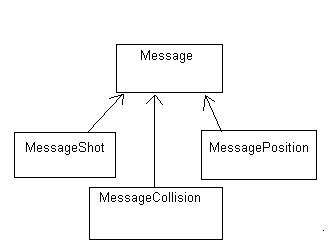
\includegraphics{pics/message.jpg}

Przed wysłaniem klasa jest zamieniana na obiekt typu string, a po odebraniu zamieniana z powrotem na odpowiedni typ. Umożliwia to proste korzystanie z systemowych gniazd TCP.

\section{Instalacja systemu}

% This section describes one or more physical network (hardware)
% configurations on which the software is deployed and run. It is a view of
% the Deployment Model. At a minimum for each configuration it should
% indicate the physical nodes (computers, CPUs) that execute the software,
% and their interconnections (bus, LAN, point-to-point, and so on.) Also
% include a mapping of the processes of the Process View onto the physical
% nodes.

Gra jest tworzona pod system Windows. Do zainstalowania i uruchomienia gry będzie zatem potrzebny komputer z zainstalowanym systemem Windows oraz stosunkowo szybki procesor, aczkolwiek nie z najwyższej półki, wraz z kartą graficzną wspomagającą grafikę 3D. Aby cieszyć się grą w trybie multiplayer (niestety tylko taki tryb gry jest póki co przewidziany) potrzebna będzie karta sieciowa wraz z poprawnie skonfigurowaną siecią lokalną, bądź dostępem do internetu.

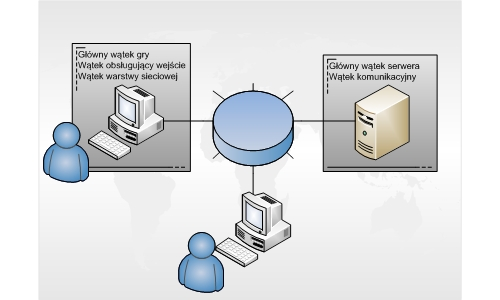
\includegraphics{pics/physicalNodes.jpg}

\section{Implementacja systemu}

% This section describes the overall structure of the implementation model,
% the decomposition of the software into layers and subsystems in the
% implementation model, and any architecturally significant components.

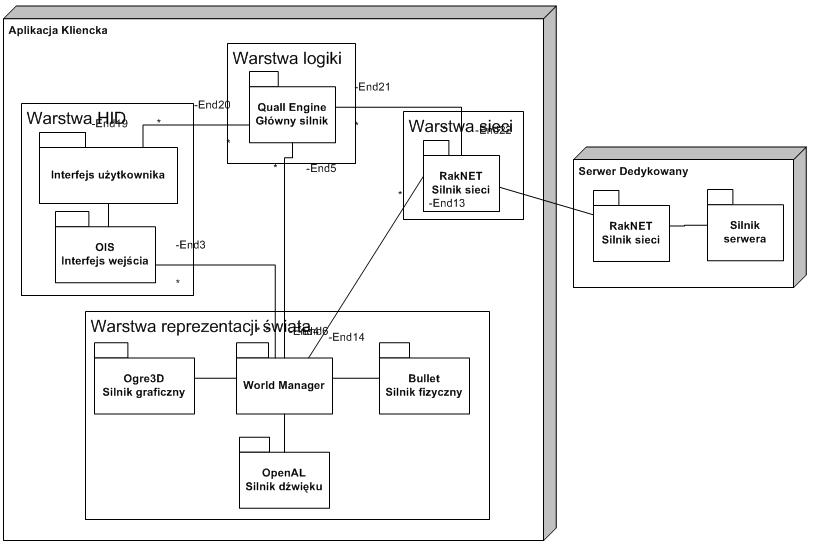
\includegraphics{pics/ModuleCommunication.jpg}

\subsection{Omówienie}

% This subsection names and defines the various layers and their contents,
% the rules that govern the inclusion to a given layer, and the boundaries
% between layers. Include a component diagram that shows the relations
% between layers. 

\subsubsection{Aplikacja kliencka}

Rozróżniamy 4 podstawowe warstwy aplikacji. Najważniejszą stanowi warstwa silnika gry. Tworzy ona wszystkie niezbędne byty i przekazuje do niższych warstw. Warstwa sieci oraz HID stanowią warstwę wejścia, która z kolei przekazuje wszystkie zdarzenia (np. kliknięcie, lub informacje od serwera) do warstwy reprezentacji świata. Ta warstwa natomiast synchronizuje wszystkie wydarzenia i następnie je wyświetla.
\subsubsection{Serwer dedykowany}
Serwer posiada dwie warstwy - sieci oraz logiczną. Serwer przelicza wydarzenia fizyczne a następnie przesyła je do innych klientów.

\subsection{Warstwy}

% For each layer, include a subsection with its name, an enumeration of the
% subsystems located in the layer, and a component diagram.

\subsubsection{Warstwa reprezentacji świata}

Do implementacji warstwy reprezantacji świata zostaną użyte 3 główne biblioteki:

\begin{itemize}
\item Bullet - służy do implementowania grawitacji, detekcji kolizji i w ogólności do wszystkich aspektów związanych z fizyką.
\item Ogre3d - biblioteka służąca do tworzenia grafiki 3d, to głównie ona będzie odpowiedzialna za to co użytkownik będzie widział na ekranie.
\item OpenAL - służy do obsługi wszystkich efektów dźwiękowych gry, takich jak odgłosy strzelania czy chodzenia, z uwzględnieniem odległości i położenia źródła.
\end{itemize}

\subsubsection{Warstwa HID}

Do implementacji tej warstwy zostanie użyta biblioteka OIS, obsługująca asynchroniczne wejście za pomocą zdarzeń. 

\subsubsection{Warstwa sieci}

Komunikacja sieciowa opiera się na protokole TCP/IP, a do jej obsługi będą użyte standardowe biblioteki systemu Windows. Do implementacji tej warstwy należy także klasa Message, która jest wymieniana pomiędzy klientem a serwerem.

%\section{Przechowywane dane}
% opcjonalnie

% A description of the persistent data storage perspective of the system.
% This section is optional if there is little or no persistent data, or the
% translation between the Design Model and the Data Model is trivial.

%\section{Wydajność systemu}

% A description of the major dimensioning characteristics of the software
% that impact the architecture, as well as the target performance
% constraints.

%\section{Jakość}

% A description of how the software architecture contributes to all
% capabilities (other than functionality) of the system: extensibility,
% reliability, portability, and so on. If these characteristics have
% special significance, for example safety, security or privacy
% implications, they should be clearly delineated.

\section{Historia zmian}

\begin{verbatim}

$Log: sad-template.tex,v $
11 XI 09 - opis architektury.
6 XII 09 - zmiana architektury logicznej.
9 XII 09 - dodanie implementacji systemu, wersja wstępna.
16 XII 09 - opis implementacji systemu.
9 I 10 - dokładniejszy opis przypadków użycia, opis protokołu komunikacyjnego między procesami, liczne poprawki i uzupełnienia treści.

\end{verbatim}

\end{document}

